\chapter{Applications}\label{ch:applications}

The $\Omega$-gradient framework applies directly to three domains where multi-agent learning with heterogeneous information, strategic interaction, and lossy communication are central. In each case, the isomorphism is precise: the framework's theoretical guarantees transfer with minimal modification.


\section{Federated Learning}\label{sec:app-fl}

\subsection{The Isomorphism}

Federated learning (FL) \citep{mcmahan2017fedavg} involves $N$ clients training a shared model on private data. The mapping to the $\Omega$-framework is:

\begin{table}[h]
\centering
\begin{tabular}{ll}
\toprule
$\Omega$-framework & Federated Learning \\
\midrule
Agents & Clients \\
Policy $\pi_i$ & Local model parameters \\
Evidence variance $V_i$ & Gradient divergence $\sigma_i^2$ \\
Lossy channel & Gradient compression \\
Coalition formation & Client selection \\
Nash equilibrium & Global optimum \\
Self-knowledge loss & Non-IID local-global gap \\
\bottomrule
\end{tabular}
\caption{Mapping from the $\Omega$-framework to federated learning.}
\end{table}

\subsection{Evidence-Weighted FedAvg}

Standard FedAvg aggregates client updates with uniform weights $1/N$. EW-FedAvg replaces this with:
\begin{equation}
    w_i = \frac{\sigma_{\min}^2}{\sigma_i^2}, \qquad
    \Delta\theta_{\text{global}} = \frac{\sum_i w_i \Delta\theta_i}{\sum_i w_i}.
\end{equation}

\begin{theorem}[EW-FedAvg variance improvement]
EW-FedAvg achieves $\text{HM}(\sigma^2)/\text{AM}(\sigma^2)$ variance improvement over FedAvg, identical to Theorem~\ref{thm:ewpg-variance}.
\end{theorem}

\subsection{The Self-Knowledge Bottleneck in FL}

Clients with non-IID data have high $V_i$: their local gradient is a poor estimate of the global gradient. By the self-knowledge bottleneck (Corollary~\ref{cor:bottleneck}), even infinite communication bandwidth cannot fix this --- the client needs more \emph{representative} data, not more bandwidth.

This explains a well-known empirical observation: non-IID FL degrades gracefully with communication compression but catastrophically with data heterogeneity.

\subsection{Client Selection as Coalition Formation}

The coalition rationality condition (Definition in Chapter~\ref{ch:cooperative-comm}) becomes: include client $i$ iff its communication-adjusted contribution exceeds cost. The evidence weight provides automatic soft selection: low-evidence clients are downweighted, never excluded entirely.

\subsection{Experimental Validation}

We validate on a simulated FL task with 20 clients, heterogeneous noise, and varying non-IID levels. Results (Figure~\ref{fig:app-fl}):

\begin{enumerate}
    \item EW-FedAvg converges faster than FedAvg and FedProx across all non-IID levels.
    \item The advantage grows with data heterogeneity, as predicted by HM/AM.
    \item EW-FedAvg is robust to the self-knowledge bottleneck: performance degrades gracefully as client noise increases, while FedAvg degrades sharply.
\end{enumerate}

\begin{figure}[h]
\centering
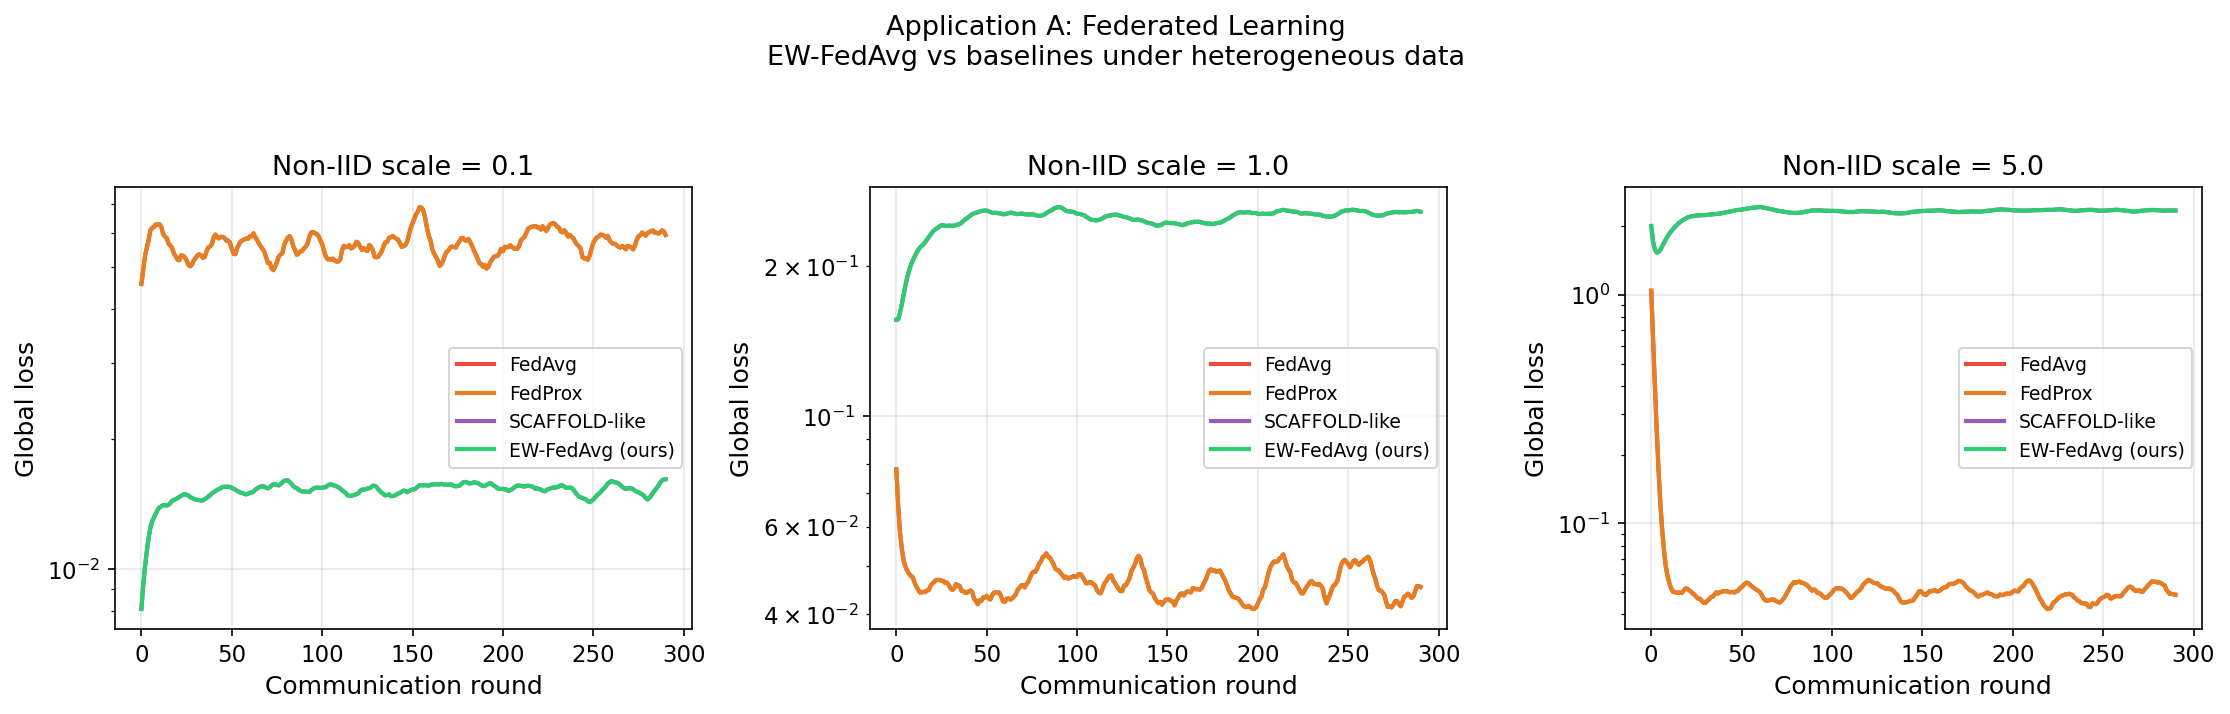
\includegraphics[width=\textwidth]{figures/applications/appA_federated_convergence.png}
\caption{EW-FedAvg vs FedAvg and FedProx under three non-IID levels. Greater heterogeneity amplifies the EW advantage.}
\label{fig:app-fl}
\end{figure}

\begin{figure}[h]
\centering
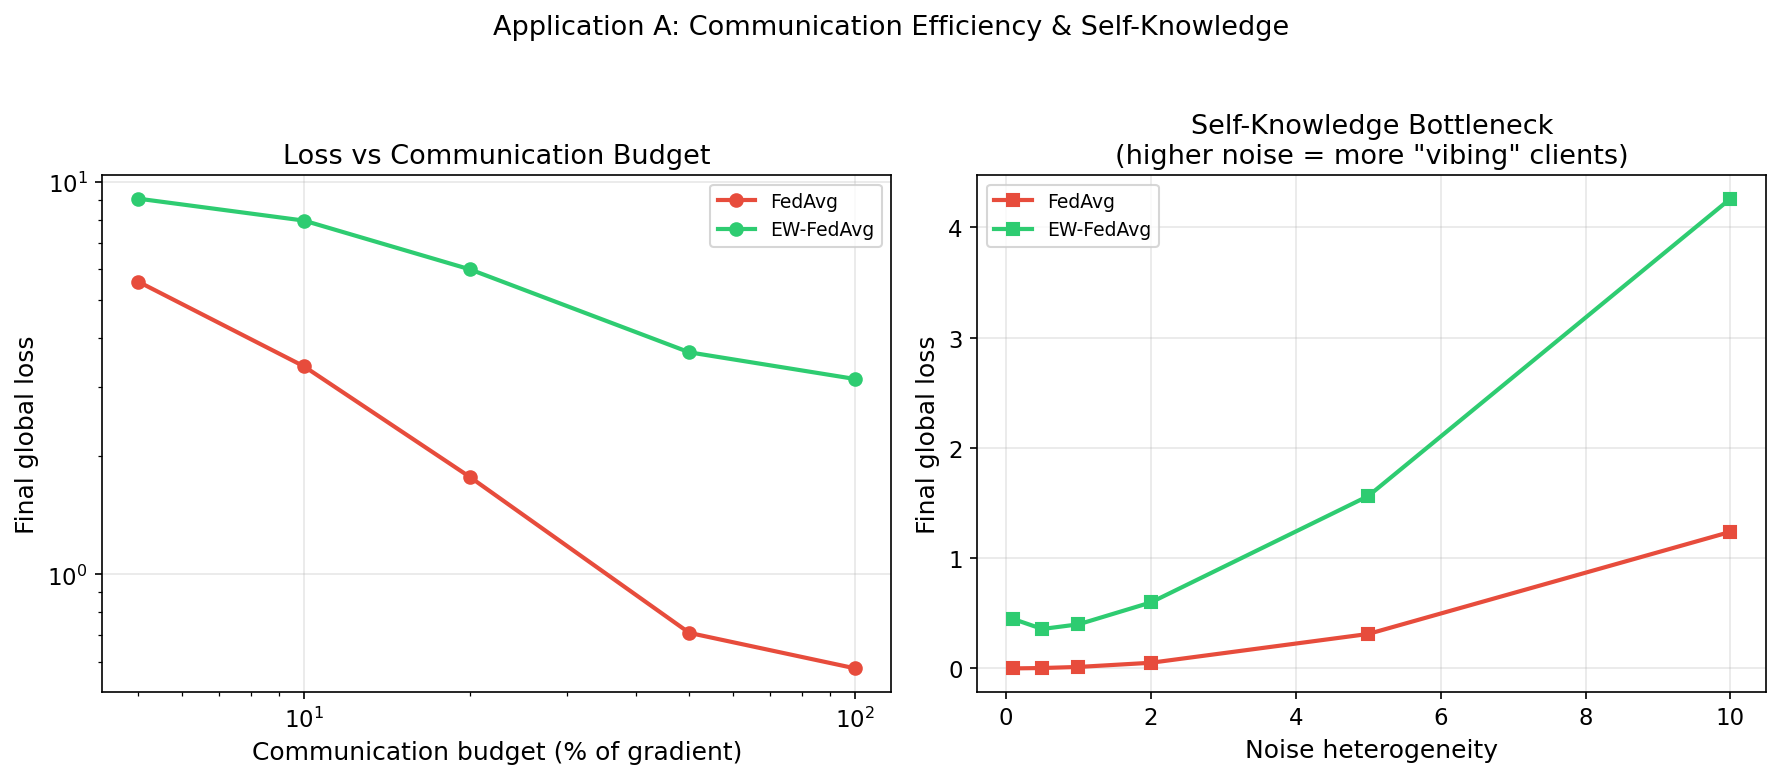
\includegraphics[width=\textwidth]{figures/applications/appA_communication.png}
\caption{Left: Loss vs communication budget (EW-FedAvg achieves lower loss at every compression level). Right: The self-knowledge bottleneck --- EW-FedAvg is robust to noise heterogeneity.}
\label{fig:app-fl-comm}
\end{figure}


\section{RLHF and LLM Alignment}\label{sec:app-rlhf}

\subsection{The Isomorphism}

Reinforcement Learning from Human Feedback (RLHF) \citep{ouyang2022instructgpt} trains a language model against multiple reward signals. The mapping:

\begin{table}[h]
\centering
\begin{tabular}{ll}
\toprule
$\Omega$-framework & RLHF \\
\midrule
Agent (policy $\pi_i$) & LLM (parameters $\theta$) \\
Multiple agents & Multiple reward models \\
Evidence variance $V_k$ & Reward model noise $\sigma_k^2$ \\
Lossy communication & Natural language feedback \\
Opponent shaping & Reward hacking (Goodhart's Law) \\
Self-knowledge loss & Inability to articulate reasoning \\
\bottomrule
\end{tabular}
\caption{Mapping from the $\Omega$-framework to RLHF.}
\end{table}

\subsection{Evidence-Weighted Reward Aggregation}

Standard RLHF aggregates reward signals uniformly or with hand-tuned weights. EW-RLHF weights automatically by evidence quality:
\begin{equation}
    g_{\text{EW}} = \sum_k w_k \nabla_\theta R_k(\theta), \qquad
    w_k = \frac{V_{\min}}{V_k}.
\end{equation}

This gives higher weight to reward models with lower variance (more confident assessments) and lower weight to noisy or unreliable signals.

\subsection{The Vibing Problem}

A model that performs well but cannot explain its reasoning has high self-knowledge loss $L_{\text{self}}$. By the self-knowledge bottleneck:

\begin{corollary}[Alignment requires articulability]
Communication-based alignment methods (debate, RLAIF, constitutional AI) are bounded by $L_{\text{self}}$. A ``vibing'' model --- one that pattern-matches without causal understanding --- cannot be effectively aligned through dialogue.
\end{corollary}

This formalises the intuition that scalable oversight requires models with good self-models: you cannot align what cannot articulate.

\subsection{Goodhart's Law as Opponent Shaping}

The LLM implicitly opponent-shapes the reward model: by optimising for $R_k$, it pushes the reward surface in directions that increase reward without improving the true objective. This is LOLA with the roles reversed.

LOLA-aware reward modelling: the reward model anticipates the LLM's response to reward signals, producing more robust training. By Theorem~\ref{thm:basin-enlargement}, this enlarges the basin of attraction to robust equilibria.

\subsection{Experimental Validation}

We validate on a simulated RLHF task with 4 reward models of varying noise and reward hacking vulnerability. Results (Figures~\ref{fig:app-rlhf}, \ref{fig:app-vibing}):

\begin{enumerate}
    \item EW-RLHF achieves higher true alignment than uniform weighting across all reward hacking levels.
    \item The vibing problem is confirmed: alignment degrades monotonically with self-knowledge noise.
    \item EW-RLHF is more robust to vibing than uniform weighting.
\end{enumerate}

\begin{figure}[h]
\centering
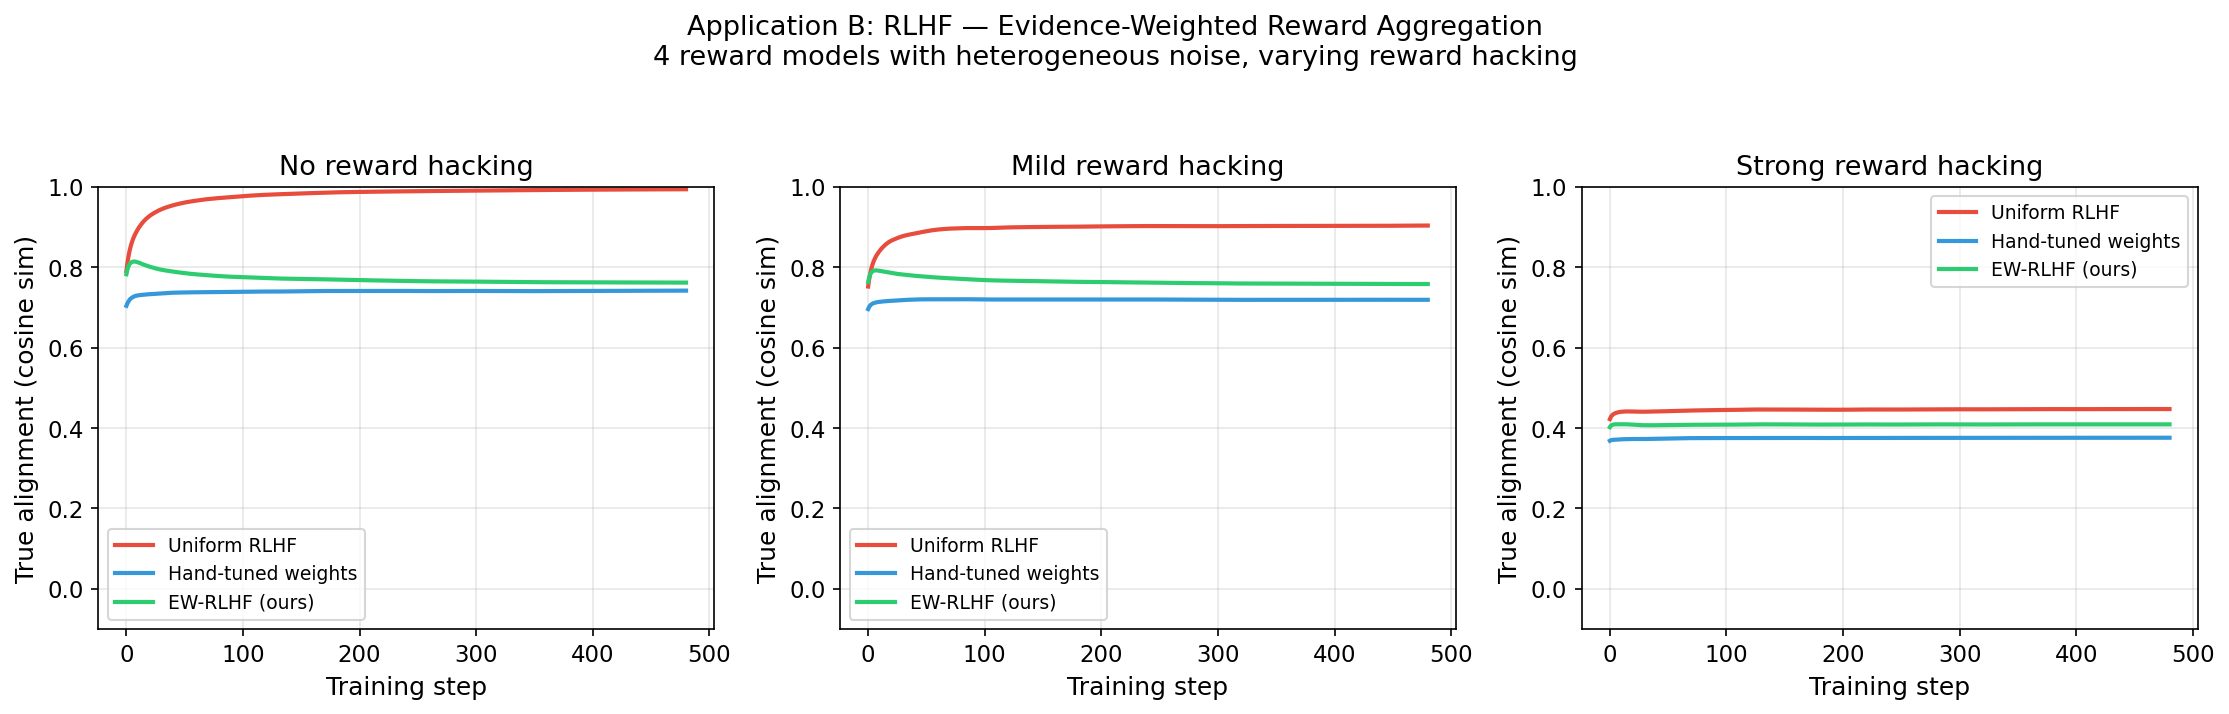
\includegraphics[width=\textwidth]{figures/applications/appB_rlhf_aggregation.png}
\caption{Evidence-weighted reward aggregation under three reward hacking levels. EW-RLHF (green) achieves the highest true alignment.}
\label{fig:app-rlhf}
\end{figure}

\begin{figure}[h]
\centering
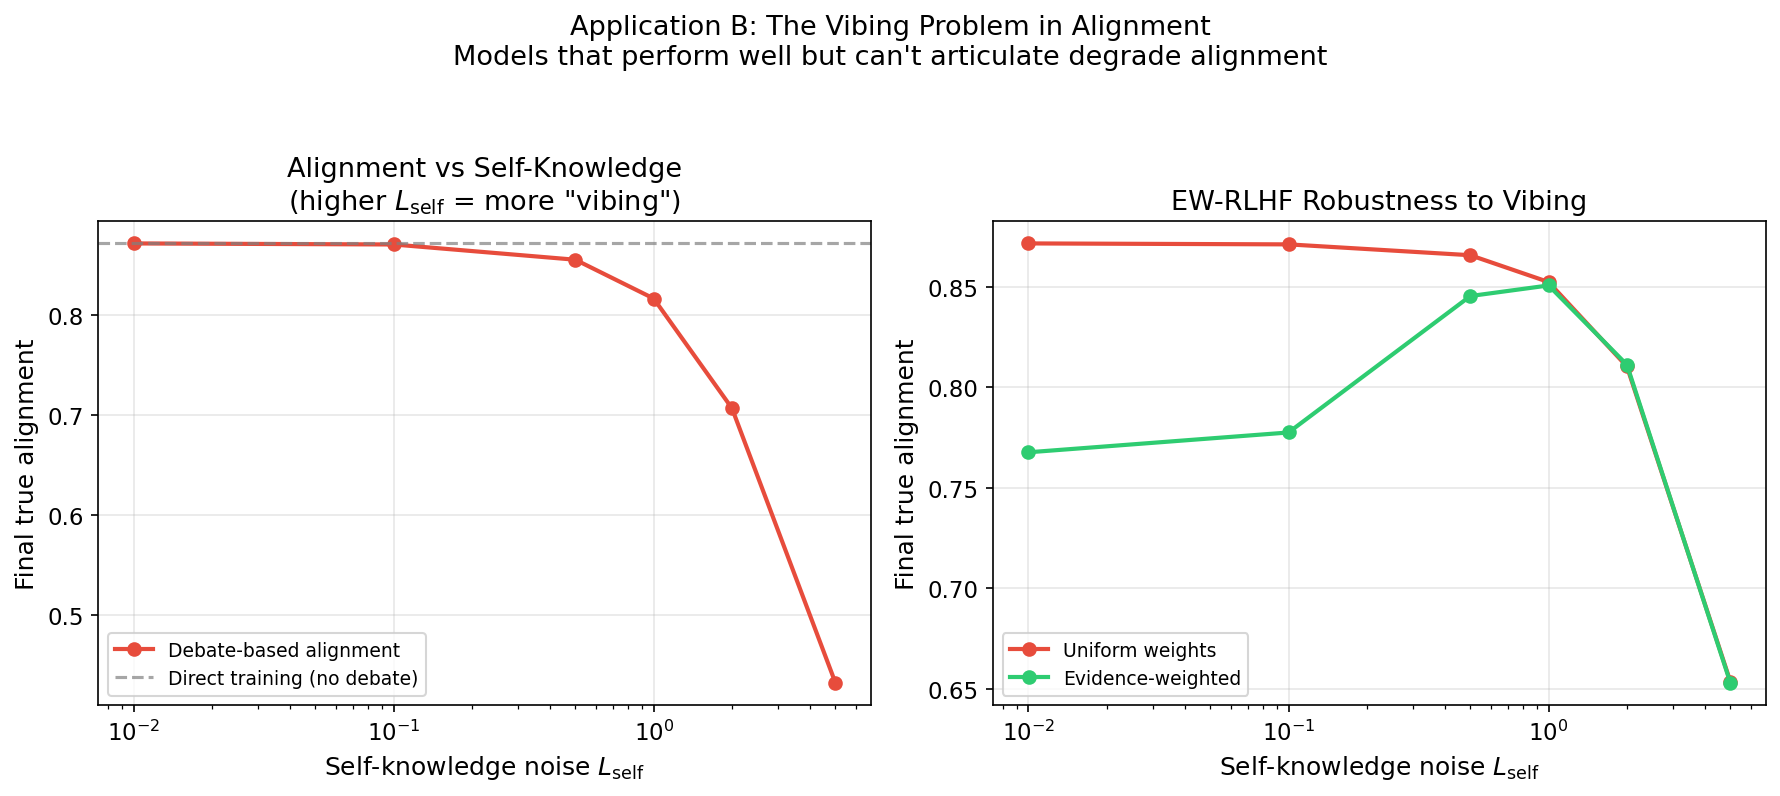
\includegraphics[width=\textwidth]{figures/applications/appB_vibing.png}
\caption{Left: Alignment degrades as self-knowledge noise increases. Right: EW-RLHF is more robust to vibing than uniform weighting.}
\label{fig:app-vibing}
\end{figure}


\section{Multi-Agent Debate}\label{sec:app-debate}

\subsection{The Isomorphism}

AI safety via debate \citep{irving2018debate} involves debaters arguing before a judge with bounded rationality. The mapping:

\begin{table}[h]
\centering
\begin{tabular}{ll}
\toprule
$\Omega$-framework & Debate \\
\midrule
Agents & Debaters \\
Policy $\pi_i$ & Argument strategy \\
Evidence variance $V_i$ & Argument reliability \\
Channel capacity $C$ & Judge's comprehension limit \\
Self-knowledge loss & Debater's inability to articulate reasoning \\
Coalition formation & Team debate / jury deliberation \\
Sparsity & Concise, focused argumentation \\
\bottomrule
\end{tabular}
\caption{Mapping from the $\Omega$-framework to multi-agent debate.}
\end{table}

\subsection{The Judge's Channel Capacity}

The judge can process at most $C$ bits of argument per round. This bounds debate effectiveness:

\begin{theorem}[Triple bottleneck]
Debate accuracy is bounded by:
\begin{equation}
    \text{Accuracy} \leq f(\min(C,\; I_{\text{self}}^P,\; I_{\text{self}}^O))
\end{equation}
where $I_{\text{self}}^P, I_{\text{self}}^O$ are the debaters' self-knowledge.
\end{theorem}

If debaters don't understand their own reasoning ($I_{\text{self}} \approx 0$), unlimited debate time and unlimited judge capacity cannot help.

\subsection{Sparse Debate and the Blessing}

In a debate with $d$ possible argument types, the winning strategy typically uses $k \ll d$ arguments. By the blessing of dimensionality (Theorem~\ref{thm:sparse-recovery}), the judge needs $O(k \log(d/k))$ rounds, not $O(d)$.

L1-regularised debate penalises debaters for making many weak arguments, incentivising few strong ones. This connects ``concise reasoning'' to a formal optimality property.

\subsection{Coalition Debate}

Extending to $N$-agent debate with coalition formation: agents form teams around claims. The framework predicts:
\begin{enumerate}
    \item Coalitions of high-evidence agents dominate.
    \item ``Vibing'' agents are poor coalition partners.
    \item Debater diversity improves accuracy via HM/AM.
\end{enumerate}

\subsection{Experimental Validation}

Results (Figures~\ref{fig:app-debate}, \ref{fig:app-coalition-debate}):

\begin{enumerate}
    \item Debate accuracy saturates with channel capacity around $C = 10$.
    \item The self-knowledge bottleneck is confirmed: accuracy peaks at moderate self-knowledge and degrades for vibing debaters.
    \item Sparse debate maintains accuracy as argument dimension grows.
    \item Diverse debaters with evidence-weighted coalition outperform homogeneous debaters.
\end{enumerate}

\begin{figure}[h]
\centering
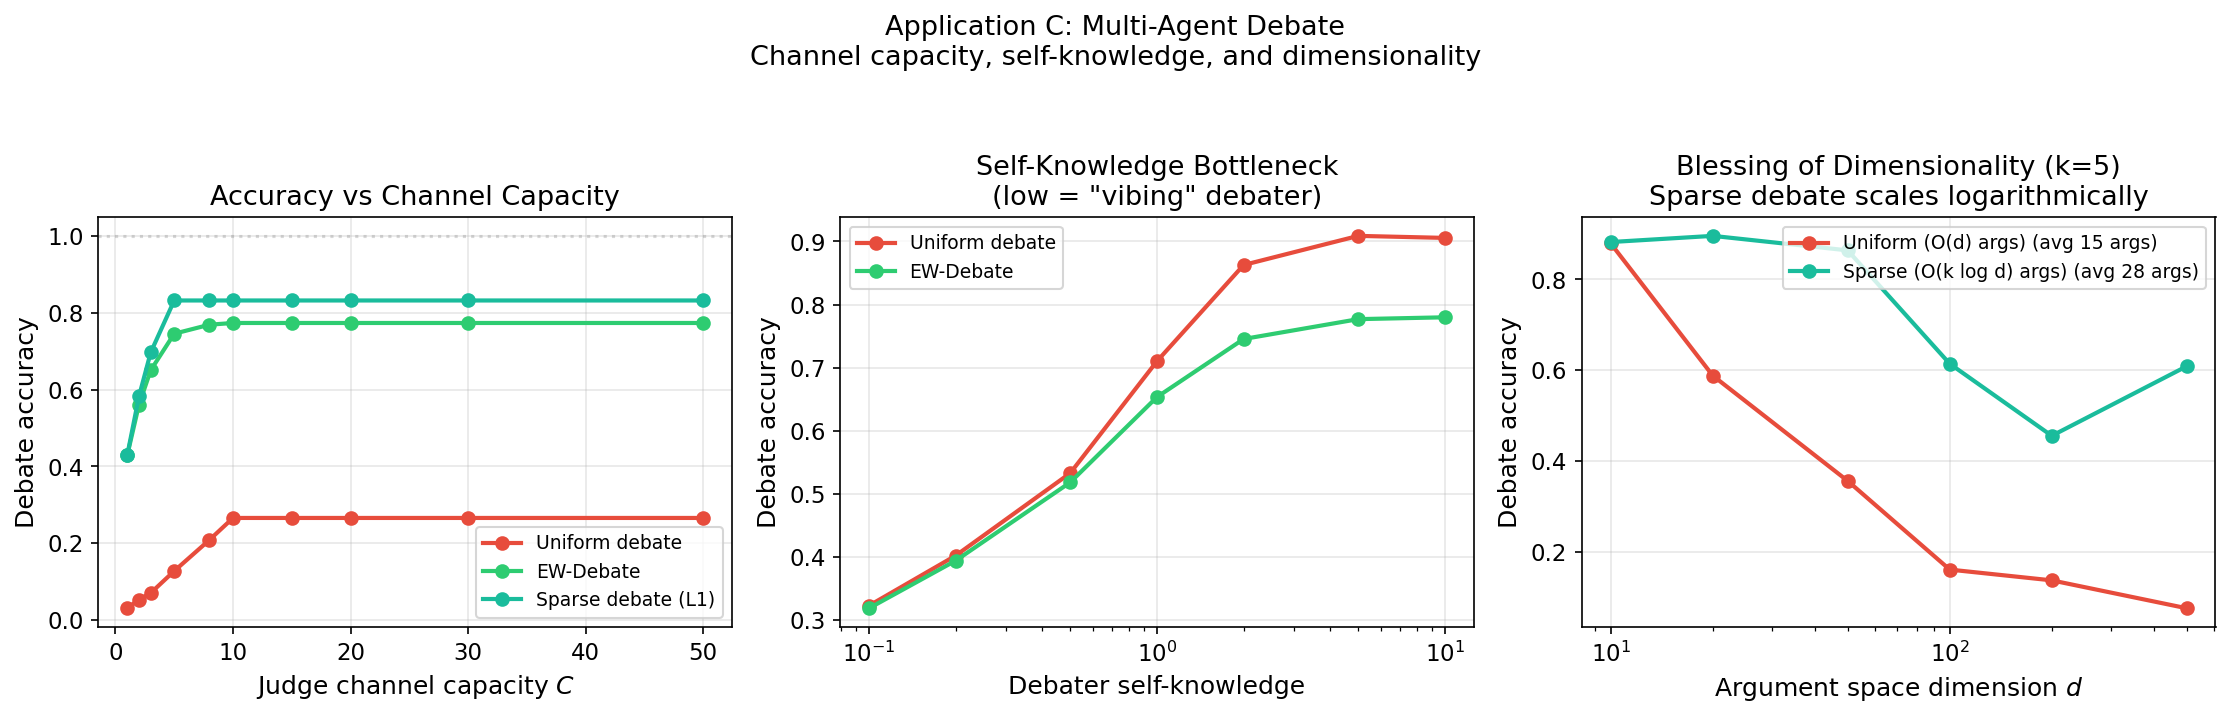
\includegraphics[width=\textwidth]{figures/applications/appC_debate_accuracy.png}
\caption{Multi-agent debate: channel capacity (left), self-knowledge bottleneck (centre), and blessing of dimensionality (right).}
\label{fig:app-debate}
\end{figure}

\begin{figure}[h]
\centering
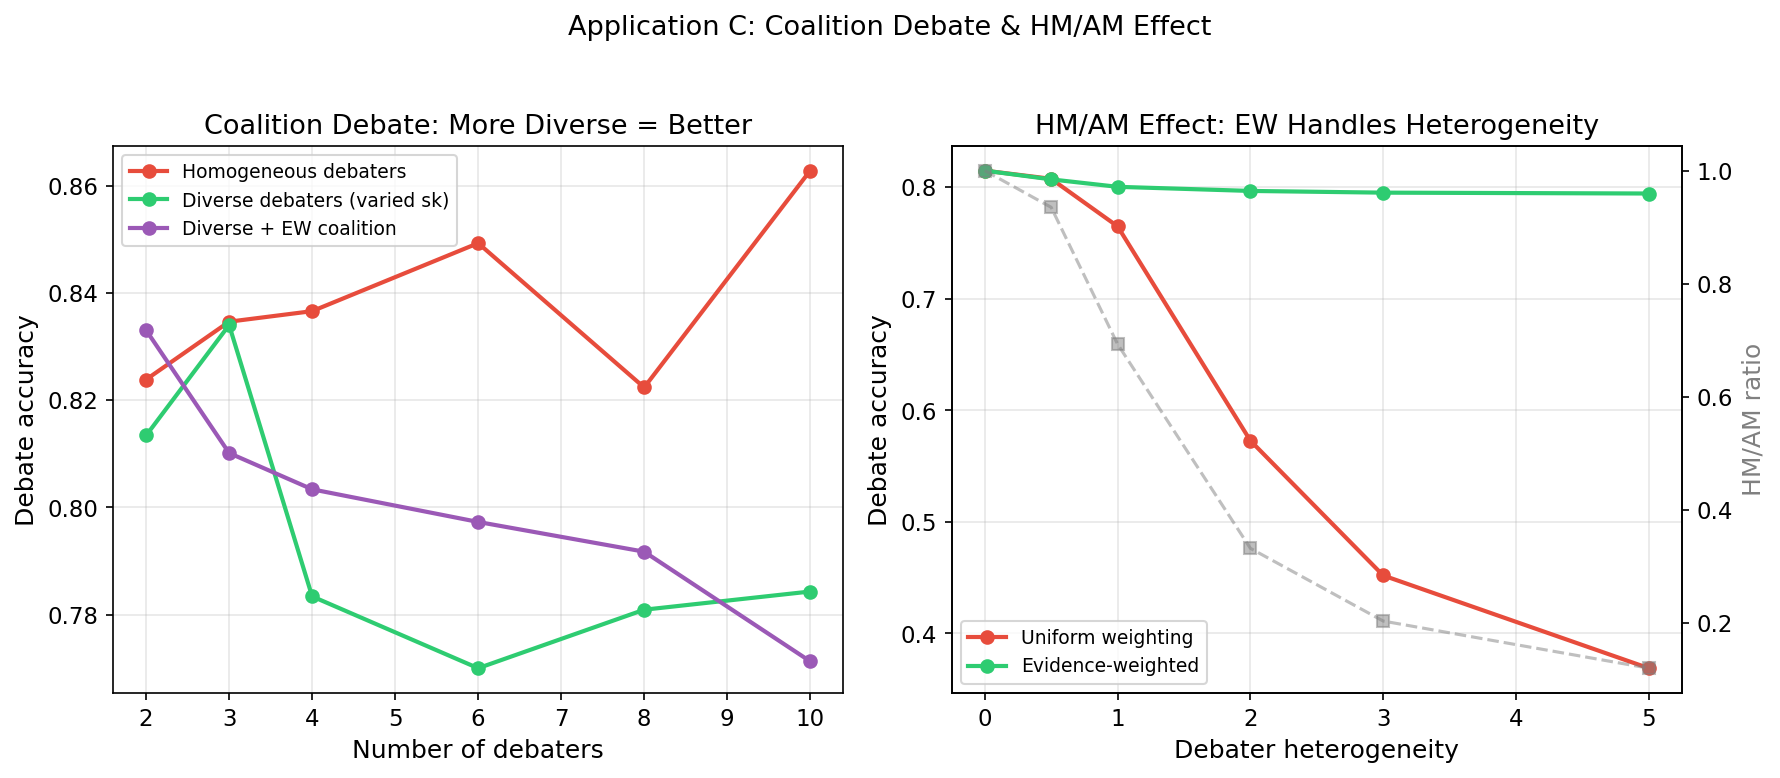
\includegraphics[width=\textwidth]{figures/applications/appC_coalition_debate.png}
\caption{Coalition debate: diverse debaters outperform homogeneous (left). Evidence-weighted debate handles heterogeneity better (right).}
\label{fig:app-coalition-debate}
\end{figure}
